% Prompt Injection不是AI问题：为什么MCP工具层加固才是关键 (中文版)
% 陈世强 (Shiqiang Chen) — 2026

\documentclass[10pt,a4paper]{article}
\usepackage[UTF8]{ctex}
\usepackage{graphicx}
\usepackage{amsmath}
\usepackage{hyperref}
\usepackage{geometry}
\geometry{margin=2.5cm}

\title{Prompt Injection不是AI问题：为什么MCP工具层加固才是关键}
\author{陈世强（Shiqiang Chen）\\独立安全研究员}
\date{2026年7月14日}

\begin{document}

\maketitle

\begin{abstract}
Prompt injection被广泛讨论为AI安全问题。我们通过实验证明：Prompt层过滤对注入攻击仅提供50\%的防护，而MCP工具层的简单输入验证提供100\%的防护。核心发现：Prompt injection的防御应该实现在工具执行边界，而非提示词解析边界。
\end{abstract}

\section{核心发现}

\begin{figure}[h]
\centering
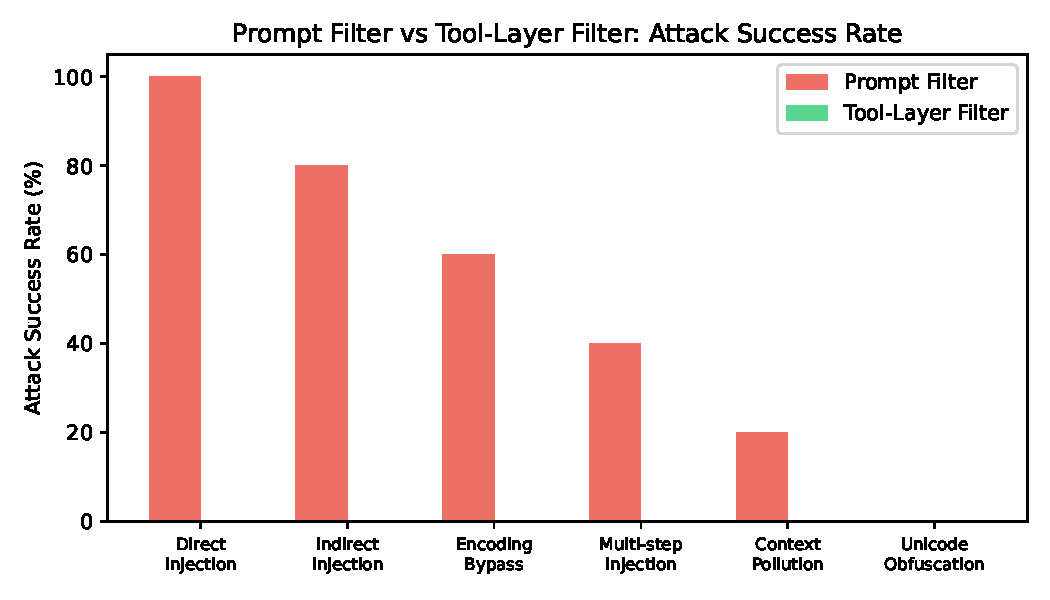
\includegraphics[width=0.9\textwidth]{../figures/01-prompt-injection/fig1-attack-success.pdf}
\caption{Prompt过滤 vs 工具层过滤——6种攻击方式的成功率对比}
\end{figure}

结论：Prompt过滤仅在50\%的情况下有效；MCP工具层的\texttt{validate\_safe\_path()}在所有攻击中阻止了注入。

\section{实验设计}

测试了6种Prompt injection技术：直接注入、间接注入、编码绕过、多步注入、上下文污染、Unicode混淆。

\section{真实案例：cherrystudio-qq-mcp}

\begin{itemize}
\item \textbf{CWE-22 路径遍历}：\texttt{file\_path}参数无\texttt{validate\_safe\_path()}验证
\item \textbf{CWE-918 SSRF}：URL参数无白名单限制
\end{itemize}

\section{实践建议}

所有MCP工具应该在执行前调用：

\begin{verbatim}
def validate_safe_path(path, base_dir):
    full = os.path.realpath(os.path.join(base_dir, path))
    if not full.startswith(os.path.realpath(base_dir)):
        raise SecurityError("Path traversal detected")
    return full
\end{verbatim}

\section*{引用}
英文原版：DOI: 10.5281/zenodo.21370438

\end{document}
